\clearpage
\cleardoublepage

\chapter{Neural Network Architectures}

\section{Introduction}

Neural network architectures define how neurons are organized and connected to process information. Different architectures are suited for different types of data and tasks. This chapter covers the three fundamental neural network architectures: Deep Neural Networks (DNN), Convolutional Neural Networks (CNN), and Recurrent Neural Networks (RNN).

\section{Deep Neural Networks (DNN)}

A Deep Neural Network consists of multiple layers of neurons, where information flows from input to output without loops.

\subsection{Architecture}

A fully-connected DNN performs:
\begin{equation}
\mathbf{h}^{(l)} = f^{(l)}(\mathbf{W}^{(l)}\mathbf{h}^{(l-1)} + \mathbf{b}^{(l)})
\end{equation}
where $l = 1, \ldots, L$ indexes the layers.

\begin{figure}[htbp]
    \centering
    \begin{tikzpicture}[scale=0.8]
        % Input layer
        \foreach \y in {1,...,4} {
            \node[circle, draw=layer-input, fill=layer-input!30] (i\y) at (0, 5-\y) {};
        }
        \node[below] at (0, 0.5) {Input};
        
        % Hidden layer 1
        \foreach \y in {1,...,5} {
            \node[circle, draw=layer-hidden, fill=layer-hidden!30] (h1\y) at (3, 5.5-\y) {};
        }
        
        % Hidden layer 2
        \foreach \y in {1,...,4} {
            \node[circle, draw=layer-hidden, fill=layer-hidden!30] (h2\y) at (6, 5-\y) {};
        }
        
        % Output layer
        \foreach \y in {1,...,2} {
            \node[circle, draw=layer-output, fill=layer-output!30] (o\y) at (9, 4.5-\y) {};
        }
        \node[below] at (9, 2) {Output};
        
        % Connections (sample)
        \foreach \i in {1,...,4} {
            \foreach \j in {1,...,5} {
                \draw[gray, opacity=0.2] (i\i) -- (h1\j);
            }
        }
        \foreach \i in {1,...,5} {
            \foreach \j in {1,...,4} {
                \draw[gray, opacity=0.2] (h1\i) -- (h2\j);
            }
        }
        \foreach \i in {1,...,4} {
            \foreach \j in {1,...,2} {
                \draw[gray, opacity=0.2] (h2\i) -- (o\j);
            }
        }
    \end{tikzpicture}
    \caption{Deep Neural Network architecture}
    \label{fig:dnn}
\end{figure}

\begin{properties}[DNN Characteristics]
\begin{itemize}
    \item \textbf{Parameter count:} $\sum_{l=1}^{L} (n^{(l-1)} \cdot n^{(l)} + n^{(l)})$
    \item \textbf{Universal approximation:} Can approximate any continuous function with sufficient width/depth
    \item \textbf{Suitable for:} Tabular data, feature-based classification
\end{itemize}
\end{properties}

\section{Convolutional Neural Networks (CNN)}

CNNs exploit spatial structure in data through local connections and parameter sharing.

\subsection{Convolutional Layer}

The convolution operation:
\begin{equation}
y[i,j] = \sum_{m}\sum_{n} w[m,n] \cdot x[i+m, j+n]
\end{equation}

\begin{figure}[htbp]
    \centering
    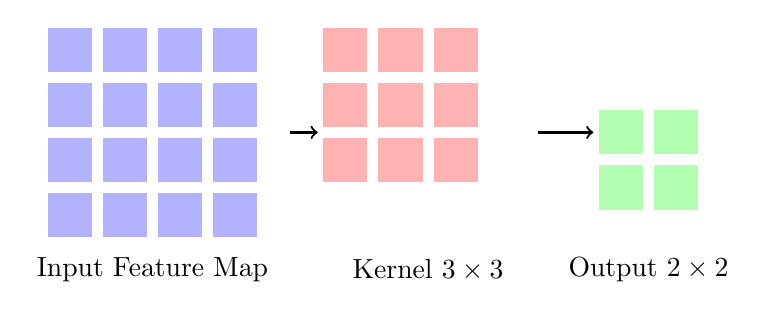
\begin{tikzpicture}[scale=0.7]
        % Input feature map
        \foreach \x in {0,...,3} {
            \foreach \y in {0,...,3} {
                \fill[blue!30] (\x, \y) +(-0.4, -0.4) rectangle ++(0.4, 0.4);
            }
        }
        \node at (1.5, -1) {Input Feature Map};
        
        % Kernel
        \foreach \x in {0,...,2} {
            \foreach \y in {0,...,2} {
                \fill[red!30] (5+\x, 1+\y) +(-0.4, -0.4) rectangle ++(0.4, 0.4);
            }
        }
        \node at (6.5, -1) {Kernel $3 \times 3$};
        
        % Output
        \foreach \x in {0,...,1} {
            \foreach \y in {0,...,1} {
                \fill[green!30] (10+\x, 0.5+\y) +(-0.4, -0.4) rectangle ++(0.4, 0.4);
            }
        }
        \node at (10.5, -1) {Output $2 \times 2$};
        
        % Arrows
        \draw[->, thick] (4, 1.5) -- (4.5, 1.5);
        \draw[->, thick] (8.5, 1.5) -- (9.5, 1.5);
    \end{tikzpicture}
    \caption{Convolution operation}
    \label{fig:convolution}
\end{figure}

Key parameters:
\begin{itemize}
    \item \textbf{Kernel size:} $K \times K$ (typically $3 \times 3$, $5 \times 5$, $7 \times 7$)
    \item \textbf{Stride:} $s$ (step size, typically 1 or 2)
    \item \textbf{Padding:} $p$ (zero-padding to control output size)
\end{itemize}

Output size:
\begin{equation}
H_{out} = \left\lfloor \frac{H_{in} + 2p - K}{s} + 1 \right\rfloor
\end{equation}

\begin{properties}[CNN Advantages]
\begin{itemize}
    \item \textbf{Local receptive field:} Each neuron sees only a local patch
    \item \textbf{Parameter sharing:} Same weights across spatial locations
    \item \textbf{Translation equivariance:} Shift in input $\rightarrow$ Shift in output
    \item \textbf{Suitable for:} Images, video, spatial data
\end{itemize}
\end{properties}

\subsection{Receptive Field Analysis}

The \textbf{receptive field} (RF) of a neuron is the region in the input image that affects its output. Understanding RF growth is crucial for architecture design.

\subsubsection{Single-Layer Receptive Field}

A single convolutional layer with kernel $K$, stride $s$, and padding $p$ produces an output whose RF is simply $K$. The output size is:
\begin{equation}
o_i = \left\lfloor \frac{i_{in} + 2p - K}{s} + 1 \right\rfloor
\end{equation}

\subsubsection{Multi-Layer Receptive Field}

For a stack of $L$ convolutional layers, the effective receptive field (ERF) of the output grows as:
\begin{equation}
\text{RF} = 1 + \sum_{l=1}^{L} \left( (K_l - 1) \cdot \prod_{l'=1}^{l-1} s_{l'} \right)
\end{equation}

\begin{example}[Two $3 \times 3$ Convolutions]
Two stacked $3 \times 3$ convolutions with stride 1:
\begin{equation}
\text{RF} = 1 + (3 - 1) \times 1 + (3 - 1) \times 1 = 5 \times 5
\end{equation}
This matches a single $5 \times 5$ convolution's receptive field, but with fewer parameters ($2 \times 9C^2$ vs $25C^2$).
\end{example}

\subsubsection{Effective Receptive Field}

While the \textbf{theoretical} receptive field covers the entire region above, the \textbf{effective} receptive field (the region that actually influences the output) has a Gaussian-like distribution centered on the receptive field center (Luo et al., 2016). Pixels near the boundary contribute significantly less to the output than those at the center.

This has important design implications:
\begin{itemize}
    \item Simply increasing the theoretical RF does not proportionally increase the effective RF
    \item Dilated/atrous convolutions can expand the effective RF without increasing parameters
    \item Deeper networks with small kernels are preferred over shallow networks with large kernels
\end{itemize}

\subsection{$1 \times 1$ Convolution: Cross-Channel Mixing}

The $1 \times 1$ convolution, also called a \textbf{pointwise convolution}, operates on each pixel independently but mixes information across channels. Despite its simplicity, it is one of the most versatile operations in modern architectures.

\textbf{Mathematical interpretation.} A $1 \times 1$ convolution with $C_{in}$ input channels and $C_{out}$ output channels is equivalent to applying a fully-connected layer at each spatial position:
\begin{equation}
y_{c_{out}}[i, j] = \sum_{c_{in}=1}^{C_{in}} w_{c_{out}, c_{in}} \cdot x_{c_{in}}[i, j] + b_{c_{out}}
\end{equation}

This can be written as a matrix multiplication: $\mathbf{Y}[i,j] = \mathbf{W} \cdot \mathbf{X}[i,j]$, where $\mathbf{W} \in \mathbb{R}^{C_{out} \times C_{in}}$.

\begin{properties}[Key Uses of $1 \times 1$ Convolution]
\begin{itemize}
    \item \textbf{Dimensionality reduction (bottleneck):} Reduce $C_{in} \to C_{in}/4$ before an expensive $3 \times 3$ convolution, then project back. Used in Inception, ResNet bottleneck, and MobileNet. Parameters: $C_{in} \times C_{out}$ (vs $K^2 \times C_{in} \times C_{out}$ for $K \times K$ conv).
    \item \textbf{Channel mixing:} Enable cross-channel information flow without spatial aggregation. Essential when features from different kernels need to interact.
    \item \textbf{Nonlinearity injection:} After each $1 \times 1$ conv, an activation function (ReLU/GELU) adds representational power. In ResNeXt and MLP-Mixer, these ``channel MLPs'' are stacked.
    \item \textbf{Depth increase without spatial cost:} Increase network depth without affecting spatial resolution or adding significant parameters.
\end{itemize}
\end{properties}

\subsection{Transposed Convolution (Deconvolution)}

For upsampling tasks (segmentation, generation), the \textbf{transposed convolution} (sometimes called deconvolution) reverses the spatial reduction of a standard convolution.

Given a standard convolution defined by stride $s$, padding $p$, and kernel $K$, the transposed convolution maps an input of size $H_{in}$ to:
\begin{equation}
H_{out} = (H_{in} - 1) \times s - 2p + K
\end{equation}

\begin{note}[Transposed Conv $\neq$ Inverse Convolution]
A transposed convolution is \textbf{not} the mathematical inverse of a convolution. It is the transpose of the convolution operator (hence the name). Given $\mathbf{Y} = \mathbf{C}\mathbf{X}$ where $\mathbf{C}$ is the convolution as a matrix, the transposed convolution computes $\mathbf{C}^\top \mathbf{Y}$. This has the same parameters but does not recover $\mathbf{X}$ exactly.
\end{note}

\section{Recurrent Neural Networks (RNN)}

RNNs process sequential data by maintaining hidden state.

\subsection{Architecture}

For input sequence $\mathbf{x}^{(1)}, \mathbf{x}^{(2)}, \ldots, \mathbf{x}^{(T)}$:
\begin{align}
\mathbf{h}^{(t)} &= f(\mathbf{W}_{xh}\mathbf{x}^{(t)} + \mathbf{W}_{hh}\mathbf{h}^{(t-1)} + \mathbf{b}_h) \\
\mathbf{y}^{(t)} &= g(\mathbf{W}_{hy}\mathbf{h}^{(t)} + \mathbf{b}_y)
\end{align}

\begin{figure}[htbp]
    \centering
    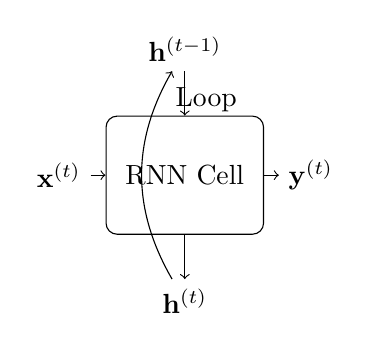
\begin{tikzpicture}[scale=0.8]
        % RNN cell
        \node[draw, minimum width=2cm, minimum height=1.5cm, rounded corners] (rnn) at (0,0) {RNN Cell};
        
        % Inputs
        \node (x) at (-2, 0) {$\mathbf{x}^{(t)}$};
        \node (h_prev) at (0, 2) {$\mathbf{h}^{(t-1)}$};
        
        % Outputs
        \node (h) at (0, -2) {$\mathbf{h}^{(t)}$};
        \node (y) at (2, 0) {$\mathbf{y}^{(t)}$};
        
        % Arrows
        \draw[->] (x) -- (rnn);
        \draw[->] (h_prev) -- (rnn);
        \draw[->] (rnn) -- (h);
        \draw[->] (rnn) -- (y);
        
        % Loop arrow
        \draw[->, bend left] (h) to (h_prev);
        \node[right] at (-0.3, 1.2) {Loop};
    \end{tikzpicture}
    \caption{RNN architecture}
    \label{fig:rnn}
\end{figure}

\begin{properties}[RNN Characteristics]
\begin{itemize}
    \item \textbf{Sequential processing:} Can handle variable-length sequences
    \item \textbf{Shared parameters:} Same weights across time steps
    \item \textbf{Memory:} Hidden state captures past information
    \item \textbf{Suitable for:} Text, time series, audio, video
\end{itemize}
\end{properties}

\begin{note}[Vanishing Gradient Problem]
Standard RNNs suffer from vanishing gradients during backpropagation through time (BPTT), making it difficult to learn long-range dependencies. This led to the development of LSTM and GRU architectures.
\end{note}

\subsection{Vanishing Gradient in RNNs: A Mathematical Proof}

Understanding \emph{why} vanilla RNNs fail on long sequences requires examining the gradient flow through time. We derive the exact condition for vanishing gradients.

\subsubsection{Backpropagation Through Time (BPTT)}

Consider the total loss over a sequence of length $T$:
\begin{equation}
\mathcal{L} = \sum_{t=1}^{T} \ell(\mathbf{y}^{(t)}, \hat{\mathbf{y}}^{(t)})
\end{equation}

The gradient of $\mathcal{L}$ with respect to $\mathbf{h}^{(k)}$ at an earlier time step $k$ involves a chain of Jacobians:
\begin{equation}
\frac{\partial \mathcal{L}}{\partial \mathbf{h}^{(k)}} = \frac{\partial \mathcal{L}}{\partial \mathbf{h}^{(T)}} \prod_{t=k+1}^{T} \frac{\partial \mathbf{h}^{(t)}}{\partial \mathbf{h}^{(t-1)}}
\end{equation}

The Jacobian of the hidden state transition (with $\mathbf{h}^{(t)} = \tanh(\mathbf{W}_{hh}\mathbf{h}^{(t-1)} + \mathbf{W}_{xh}\mathbf{x}^{(t)} + \mathbf{b})$) is:
\begin{equation}
\frac{\partial \mathbf{h}^{(t)}}{\partial \mathbf{h}^{(t-1)}} = \text{diag}\bigl(1 - (\mathbf{h}^{(t)})^2\bigr) \cdot \mathbf{W}_{hh}
\end{equation}

\subsubsection{Spectral Analysis}

The product of $T - k$ Jacobians can be analyzed through their spectral properties:
\begin{equation}
\left\| \prod_{t=k+1}^{T} \frac{\partial \mathbf{h}^{(t)}}{\partial \mathbf{h}^{(t-1)}} \right\| \leq \prod_{t=k+1}^{T} \left\| \frac{\partial \mathbf{h}^{(t)}}{\partial \mathbf{h}^{(t-1)}} \right\| \leq \prod_{t=k+1}^{T} \gamma_t
\end{equation}
where $\gamma_t = \lambda_{\max}\bigl(\mathbf{W}_{hh}\bigr) \cdot \sup_i |1 - (h_i^{(t)})^2| \leq \lambda_{\max}\bigl(\mathbf{W}_{hh}\bigr)$ since $|1 - \tanh^2(x)| \leq 1$.

\begin{theorem}[Vanishing/Exploding Gradient Condition]
The gradient through time satisfies:
\begin{equation}
\left\| \frac{\partial \mathcal{L}}{\partial \mathbf{h}^{(k)}} \right\| \approx \left\| \frac{\partial \mathcal{L}}{\partial \mathbf{h}^{(T)}} \right\| \cdot \gamma^{T-k}
\end{equation}
where $\gamma = \lambda_{\max}(\mathbf{W}_{hh})$. Therefore:
\begin{itemize}
    \item If $\gamma < 1$: gradient \textbf{vanishes} exponentially as $\gamma^{T-k} \to 0$
    \item If $\gamma > 1$: gradient \textbf{explodes} exponentially
    \item If $\gamma = 1$ (on the boundary): gradient is preserved, but this is a measure-zero condition
\end{itemize}
\end{theorem}

\begin{properties}[Why This Matters in Practice]
\begin{itemize}
    \item Typical random initialization yields $\gamma \ll 1$ with high probability (Bengio et al., 1994)
    \item For a sequence of length $T = 100$ and $\gamma = 0.9$: gradient magnitude $\approx 0.9^{100} \approx 2.7 \times 10^{-5}$ --- effectively zero
    \item The eigenvalues of $\mathbf{W}_{hh}$ are clipped to $[-1, 1]$ by the $\tanh$ derivative, pushing toward vanishing
    \item This is fundamentally a \textbf{dynamical systems} problem: the RNN is a discrete-time dynamical system whose fixed points are either attractive ($\gamma < 1$) or repulsive ($\gamma > 1$)
\end{itemize}
\end{properties}

\section{Long Short-Term Memory (LSTM)}

LSTM addresses the vanishing gradient problem with gating mechanisms.

\subsection{LSTM Gates}

\begin{align}
\mathbf{f}^{(t)} &= \sigma(\mathbf{W}_f[\mathbf{h}^{(t-1)}, \mathbf{x}^{(t)}] + \mathbf{b}_f) \quad \text{(forget gate)} \\
\mathbf{i}^{(t)} &= \sigma(\mathbf{W}_i[\mathbf{h}^{(t-1)}, \mathbf{x}^{(t)}] + \mathbf{b}_i) \quad \text{(input gate)} \\
\mathbf{o}^{(t)} &= \sigma(\mathbf{W}_o[\mathbf{h}^{(t-1)}, \mathbf{x}^{(t)}] + \mathbf{b}_o) \quad \text{(output gate)} \\
\tilde{\mathbf{c}}^{(t)} &= \tanh(\mathbf{W}_c[\mathbf{h}^{(t-1)}, \mathbf{x}^{(t)}] + \mathbf{b}_c) \quad \text{(cell candidate)} \\
\mathbf{c}^{(t)} &= \mathbf{f}^{(t)} \odot \mathbf{c}^{(t-1)} + \mathbf{i}^{(t)} \odot \tilde{\mathbf{c}}^{(t)} \quad \text{(cell state)} \\
\mathbf{h}^{(t)} &= \mathbf{o}^{(t)} \odot \tanh(\mathbf{c}^{(t)}) \quad \text{(hidden state)}
\end{align}

\begin{figure}[htbp]
    \centering
    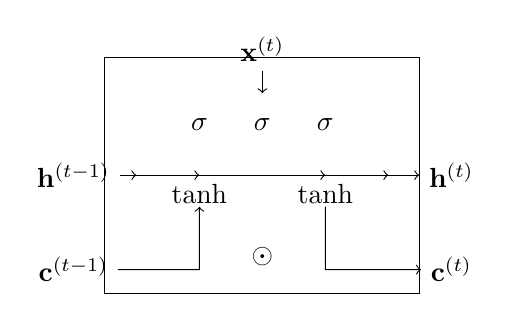
\begin{tikzpicture}[scale=0.8]
        % LSTM cell representation
        \node[draw, rectangle, minimum width=4cm, minimum height=3cm] (lstm) at (0,0) {};
        
        % Internal structure
        \node at (-1, 0.8) {$\sigma$};
        \node at (0, 0.8) {$\sigma$};
        \node at (1, 0.8) {$\sigma$};
        \node at (-1, -0.3) {$\tanh$};
        \node at (1, -0.3) {$\tanh$};
        
        % Labels
        \node at (0, -1.3) {$\odot$};
        
        % Inputs/Outputs
        \node (h_prev) at (-3, 0) {$\mathbf{h}^{(t-1)}$};
        \node (x) at (0, 2) {$\mathbf{x}^{(t)}$};
        \node (h) at (3, 0) {$\mathbf{h}^{(t)}$};
        \node (c_prev) at (-3, -1.5) {$\mathbf{c}^{(t-1)}$};
        \node (c) at (3, -1.5) {$\mathbf{c}^{(t)}$};
        
        % Arrows
        \draw[->] (h_prev) -- (-2, 0);
        \draw[->] (x) -- (0, 1.3);
        \draw[->] (-2, 0) -- (-1, 0);
        \draw[->] (-1, 0) -- (1, 0);
        \draw[->] (1, 0) -- (2, 0);
        \draw[->] (2, 0) -- (h);
        \draw[->] (c_prev) -- (-1, -1.5) -- (-1, -0.5);
        \draw[->] (1, -0.5) -- (1, -1.5) -- (2, -1.5) -- (c);
    \end{tikzpicture}
    \caption{LSTM cell structure}
    \label{fig:lstm}
\end{figure}

\begin{properties}[LSTM Advantages]
\begin{itemize}
    \item \textbf{Selective memory:} Gates control what to remember/forget
    \item \textbf{Long-range dependencies:} Cell state enables gradient flow
    \item \textbf{Widely used:} NLP, speech, time series
\end{itemize}
\end{properties}

\subsection{Why LSTM Solves the Vanishing Gradient}

The key insight is that the cell state $\mathbf{c}^{(t)}$ provides an \textbf{additive} (rather than multiplicative) path for gradient flow.

\subsubsection{Gradient Flow Through the Cell State}

Unlike the vanilla RNN where $\mathbf{h}^{(t)} = f(\mathbf{W}_{hh}\mathbf{h}^{(t-1)} + \cdots)$, the LSTM cell state updates via addition:
\begin{equation}
\mathbf{c}^{(t)} = \mathbf{f}^{(t)} \odot \mathbf{c}^{(t-1)} + \mathbf{i}^{(t)} \odot \tilde{\mathbf{c}}^{(t)}
\end{equation}

The gradient of the loss with respect to the cell state at time $k$ is:
\begin{equation}
\frac{\partial \mathcal{L}}{\partial \mathbf{c}^{(k)}} = \frac{\partial \mathcal{L}}{\partial \mathbf{c}^{(T)}} \prod_{t=k+1}^{T} \left( \mathbf{f}^{(t)} \odot \frac{\partial \mathbf{c}^{(t)}}{\partial \mathbf{c}^{(t-1)}} + \cdots \right)
\end{equation}

The critical Jacobian is:
\begin{equation}
\frac{\partial \mathbf{c}^{(t)}}{\partial \mathbf{c}^{(t-1)}} = \text{diag}\bigl(\mathbf{f}^{(t)}\bigr)
\end{equation}

When the forget gate $\mathbf{f}^{(t)} \approx \mathbf{1}$ (which the network can learn to set), the gradient is \textbf{passed through with near-identity mapping}:
\begin{equation}
\frac{\partial \mathcal{L}}{\partial \mathbf{c}^{(k)}} \approx \frac{\partial \mathcal{L}}{\partial \mathbf{c}^{(T)}}
\end{equation}

\begin{properties}[Intuition: What Each Gate Does]
\begin{itemize}
    \item \textbf{Forget gate $\mathbf{f}^{(t)}$:} ``Should I erase this information?'' Values near 0 discard old content; values near 1 preserve it. This is the key to solving vanishing gradients --- the network learns when to keep information flowing.
    \item \textbf{Input gate $\mathbf{i}^{(t)}$:} ``Is this new input worth writing?'' Acts as a gate on the cell candidate. Prevents irrelevant inputs from overwriting the cell state.
    \item \textbf{Output gate $\mathbf{o}^{(t)}$:} ``Should I expose this information now?'' Controls when the cell state contributes to the hidden state. Allows the cell to store information without immediately using it.
    \item \textbf{Cell state $\mathbf{c}^{(t)}$:} The ``conveyor belt.'' Information flows along this path largely unimpeded when forget gates are near 1. This is the \textbf{information highway} that bypasses the vanishing gradient problem.
\end{itemize}
\end{properties}

\subsubsection{Comparison: RNN vs LSTM Gradient}

\begin{table}[ht]
    \centering
    \caption{Gradient Flow: Vanilla RNN vs LSTM}
    \begin{tabular}{L{4cm} L{4.5cm} L{4.5cm}}
        \toprule
        \textbf{Aspect} & \textbf{Vanilla RNN} & \textbf{LSTM} \\
        \midrule
        State update & $\mathbf{h}^{(t)} = \tanh(\mathbf{W}\mathbf{h}^{(t-1)} + \cdots)$ & $\mathbf{c}^{(t)} = \mathbf{f}^{(t)}\odot\mathbf{c}^{(t-1)} + \cdots$ \\
        Gradient path & Multiplicative & Additive + gated \\
        Jacobian & $\text{diag}(1-\mathbf{h}^2)\mathbf{W}_{hh}$ & $\text{diag}(\mathbf{f}^{(t)})$ \\
        Learning-based & No control over gradient flow & Network learns $\mathbf{f}^{(t)}$ \\
        Long-range ($T\!=\!100$) & $\gamma^{100} \approx 0$ & $1.0^{100} = 1.0$ \\
        \bottomrule
    \end{tabular}
\end{table}

\section{Gated Recurrent Unit (GRU)}

GRU simplifies LSTM with fewer gates while maintaining performance.

\subsection{GRU Equations}
\begin{align}
\mathbf{z}^{(t)} &= \sigma(\mathbf{W}_z[\mathbf{h}^{(t-1)}, \mathbf{x}^{(t)}]) \quad \text{(update gate)} \\
\mathbf{r}^{(t)} &= \sigma(\mathbf{W}_r[\mathbf{h}^{(t-1)}, \mathbf{x}^{(t)}]) \quad \text{(reset gate)} \\
\tilde{\mathbf{h}}^{(t)} &= \tanh(\mathbf{W}[\mathbf{r}^{(t)} \odot \mathbf{h}^{(t-1)}, \mathbf{x}^{(t)}]) \\
\mathbf{h}^{(t)} &= (1 - \mathbf{z}^{(t)}) \odot \mathbf{h}^{(t-1)} + \mathbf{z}^{(t)} \odot \tilde{\mathbf{h}}^{(t)}
\end{align}

Comparison with LSTM:
\begin{itemize}
    \item Fewer parameters (2 gates vs 3)
    \item No separate cell state
    \item Often performs comparably to LSTM
\end{itemize}

\section{Choosing Architecture}

\begin{table}[ht]
    \centering
    \caption{Architecture Selection Guide}
    \begin{tabular}{L{2.5cm} L{3.5cm} L{4cm}}
        \toprule
        \textbf{Architecture} & \textbf{Best For} & \textbf{Examples} \\
        \midrule
        DNN & Tabular data & Classification, regression \\
        CNN & Images, spatial data & Object detection, segmentation \\
        RNN/LSTM & Sequences & NLP, time series \\
        Transformer & Long sequences & Translation, generation \\
        \bottomrule
    \end{tabular}
\end{table}

\section{Chapter Summary}

\begin{enumerate}
    \item DNNs are fully-connected networks for general-purpose learning
    \item CNNs exploit spatial structure through local connections and parameter sharing
    \item Receptive field grows with network depth; effective RF has Gaussian-like distribution
    \item $1 \times 1$ convolutions enable efficient cross-channel mixing and dimensionality reduction
    \item RNNs process sequential data with recurrent connections
    \item Vanilla RNNs suffer from exponentially vanishing/exploding gradients ($\gamma^{T-k}$)
    \item LSTM solves this with an additive cell state pathway and learnable forget gates
    \item GRU simplifies LSTM with fewer parameters while maintaining competitive performance
    \item Architecture choice depends on data type, sequence length, and task requirements
\end{enumerate}

\section{Further Reading}

\begin{itemize}
    \item Bengio, Y., Simard, P., \& Frasconi, P. (1994). Learning long-term dependencies with gradient descent is difficult. \textit{IEEE Transactions on Neural Networks}, 5(2), 157--166.
    \item Hochreiter, S. \& Schmidhuber, J. (1997). Long short-term memory. \textit{Neural Computation}, 9(8), 1735--1780.
    \item Cho, K. et al. (2014). Learning phrase representations using RNN encoder-decoder for statistical machine translation. \textit{EMNLP}.
    \item Luo, W., Li, Y., Urtasun, R., \& Zemel, R. (2016). Understanding the effective receptive field in deep convolutional neural networks. \textit{NeurIPS}.
    \item He, K., Zhang, X., Ren, S., \& Sun, J. (2016). Deep residual learning for image recognition. \textit{CVPR}.
\end{itemize}
